\documentclass{echw}

\title{Tutorial A10C\\Complex Numbers}
\author{Eytan Chong}
\date{2024-07-07}

\begin{document}
    \problem{}
        Given that $z = 1 + i$ and $w = 1 + 2i$, mark on an Argand diagram, the positions representing: $z$, $w$, $z + w$, $z - w$, $iz$ and $2z\cconj$.

    \solution
        \begin{center}
            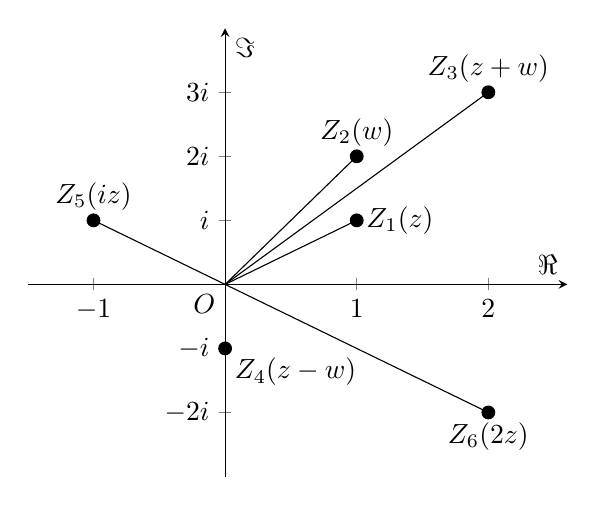
\begin{tikzpicture}[trim axis left, trim axis right]
                \begin{axis}[
                    domain = 0:10,
                    samples = 101,
                    axis y line=middle,
                    axis x line=middle,
                    xtick = {-1, 1, 2},
                    ytick = {-2, -1, 1, 2, 3},
                    yticklabels = {$-2i$, $-i$, $i$, $2i$, $3i$},
                    xmax=2.6,
                    xmin=-1.5,
                    ymin=-3,
                    ymax=4,
                    xlabel = {$\Re$},
                    ylabel = {$\Im$},
                    legend cell align={left},
                    legend pos=outer north east,
                    after end axis/.code={
                        \path (axis cs:0,0) 
                            node [anchor=north east] {$O$};
                        }
                    ]
        
                    \coordinate (R) at (10,0);
                    \coordinate[label=right:$Z_1(z)$] (Z1) at (1, 1);
                    \coordinate[label=above:$Z_2(w)$] (Z2) at (1, 2);
                    \coordinate[label=above:$Z_3(z + w)$] (Z3) at (2, 3);
                    \coordinate[label=below right:$Z_4(z - w)$] (Z4) at (0, -1);
                    \coordinate[label=above:$Z_5(iz)$] (Z5) at (-1, 1);
                    \coordinate[label=below:$Z_6(2z\cconj)$] (Z6) at (2, -2);
                    \coordinate (O) at (0, 0);
            
                    \draw (O) -- (Z1);
                    \draw (O) -- (Z2);
                    \draw (O) -- (Z3);
                    \draw (O) -- (Z4);
                    \draw (O) -- (Z5);
                    \draw (O) -- (Z6);
            
                    \fill (Z1) circle[radius=2.5pt];
                    \fill (Z2) circle[radius=2.5pt];
                    \fill (Z3) circle[radius=2.5pt];
                    \fill (Z4) circle[radius=2.5pt];
                    \fill (Z5) circle[radius=2.5pt];
                    \fill (Z6) circle[radius=2.5pt];
                \end{axis}
            \end{tikzpicture}
        \end{center}

    \problem{}
        \begin{enumerate}
            \item Write down the exact values of the modulus and the argument of the complex number $\dfrac12 + \dfrac{\sqrt3}2 i$.
            \item The complex numbers $z$ and $w$ satisfy the equation \[z^2 - zw + w^2 = 0\] Find $z$ in terms of $w$. In an Argand diagram, the points $O$, $A$ and $B$ represent the complex numbers $0$, $z$ and $w$ respectively. Show that $\triangle OAB$ is an equilateral triangle.
        \end{enumerate}

    \solution
        \part
            We have $r^2 = \bp{\dfrac12}^2 + \bp{\dfrac{\sqrt3}2}^2 \implies r = 1$ and $\tan \t = \dfrac{\sqrt3 /2}{1/2} \implies \t = \dfrac\pi3$.
            \boxt{$\abs{\dfrac12 + \dfrac{\sqrt3}2 i} = 1$, $\arg{\dfrac12 + \dfrac{\sqrt3}2 i} = \dfrac\pi3$}
        
        \part
            From the quadratic formula, we have $z = \dfrac{w \pm \sqrt{w^2 - 4w^2}}{2} = w \bp{\dfrac12 \pm \dfrac{\sqrt3}2 i}$.

            \begin{center}
                \begin{tikzpicture}[trim axis left, trim axis right]
                    \begin{axis}[
                        domain = 0:10,
                        samples = 101,
                        axis y line=middle,
                        axis x line=middle,
                        xtick = \empty,
                        ytick = \empty,
                        xmax=2,
                        xmin=-2,
                        ymin=-1.5,
                        ymax=2,
                        xlabel = {$\Re$},
                        ylabel = {$\Im$},
                        legend cell align={left},
                        legend pos=outer north east,
                        after end axis/.code={
                            \path (axis cs:0,0) 
                                node [anchor=north east] {$O$};
                            }
                        ]
            
                        \coordinate (R) at (10,0);
                        \coordinate[label=right:$B(w)$] (B) at (1, 1);
                        \coordinate[label=left:$A_1(z_1)$] (A1) at (-0.366, 1.366);
                        \coordinate[label=below:$A_2(z_2)$] (A2) at (1.366, -0.366);

                        \coordinate (O) at (0, 0);
                
                        \draw (O) -- (B);
                        \draw (O) -- (A1);
                        \draw (O) -- (A2);
                        
                        \draw[dotted] (A1) -- (B);
                        \draw[dotted] (A2) -- (B);
                
                        \fill (A1) circle[radius=2.5pt];
                        \fill (A2) circle[radius=2.5pt];
                        \fill (B) circle[radius=2.5pt];
                        \draw pic [draw, angle radius=10mm, "$\t$"] {angle = B--O--A1};
                        \draw pic [draw, angle radius=12mm, "$\t$"] {angle = A2--O--B};
                    \end{axis}
                \end{tikzpicture}
            \end{center}

            Since $\abs{\dfrac12 \pm \dfrac{\sqrt3}2 i} = 1$, we have that $OB = OA_1 = OA_2$. Further, since $\arg{\dfrac12 \pm \dfrac{\sqrt3}2 i} = \pm \dfrac\pi3$, we know $\angle A_1OB = \angle A_2OB = \dfrac\pi3$, whence $\triangle A_1OB$ and $\triangle A_2OB$ are both equilateral.

    \problem{}
        Find the exact roots of the equations
        \begin{enumerate}
            \item $z^3 = 1$
            \item $(z-1)^4 = -16$
        \end{enumerate}
        in the form $x + iy$.

    \solution
        \part
            Since $1 = e^{i2\pi n}$, $n \in \Z$, we have $z^3 = e^{i 2\pi n}$, whence $z = e^{i 2 \pi n / 3} = \cos \dfrac{2\pi n}3 + i \sin \dfrac{2\pi n}3$. Evaluating $z$ in the $n = 0, 1, 2$ cases,
            \begin{align*}
                n = 0 &: z = \cos 0 + i \sin 0 = 1\\
                n = 1 &: z = \cos \dfrac{2\pi}3 + i \sin \dfrac{2\pi}3  = -\dfrac12 + \dfrac{\sqrt3}2 i\\
                n = 2 &: z = \cos \dfrac{4\pi}3 + i \sin \dfrac{4\pi}3  = -\dfrac12 - \dfrac{\sqrt3}2 i
            \end{align*}

            \boxt{$1$, $-\dfrac12 + \dfrac{\sqrt3}2 i$, $-\dfrac12 - \dfrac{\sqrt3}2 i$}

        \part
            Observe that $-16 = 16e^{i\pi + 2\pi n} = 16e^{i\pi(2n+1)}$, $n \in \Z$. Hence,
            \begin{alignat*}{2}
                &&(z-1)^4 &= 16e^{i\pi(2n+1)}\\
                \implies&&z - 1 &= 2e^{i\pi(2n+1)/4}\\
                \implies&& z &= 1 + 2e^{i\pi(2n+1)/4}\\
                && &= 1 + 2\bs{\cos{\dfrac{2n+1}4 \pi} + i\sin{\dfrac{2n+1}4 \pi}}
            \end{alignat*}
            Evaluating $z$ in the $n = 0, 1, 2, 3$ cases,
            \begin{align*}
                n = 0 &: z = 1 + 2\bs{\cos \dfrac{\pi}4 + i \sin \dfrac{\pi}4} = (1 + \sqrt2) + i\sqrt2\\
                n = 1 &: z = 1 + 2\bs{\cos \dfrac{3\pi}4 + i \sin \dfrac{3\pi}4} = (1 - \sqrt2) + i\sqrt2\\
                n = 2 &: z = 1 + 2\bs{\cos \dfrac{5\pi}4 + i \sin \dfrac{5\pi}4} = (1 - \sqrt2) - i\sqrt2\\
                n = 3 &: z = 1 + 2\bs{\cos \dfrac{7\pi}4 + i \sin \dfrac{7\pi}4} = (1 + \sqrt2) - i\sqrt2
            \end{align*}

            \boxt{$(1 + \sqrt2) \pm i\sqrt2$, $(1 - \sqrt2) \pm i \sqrt2$}

    \problem{}
        \begin{enumerate}
            \item Write down the 5 roots of the equation $z^5 - 1 = 0$ in the form $re^{i\t}$, where $r > 0$ and $-\pi < \t \leq \pi$.
            \item Show that the roots of the equation $(5+z)^5 - (5-z)^5 = 0$ can be written in the form $5i \tan \dfrac{k\pi}5$, where $k = 0, \pm 1, \pm 2.$
        \end{enumerate}

    \solution
        \part
            Observe that $1 = e^{2\pi n}$, $n \in \Z$. Hence, $z^5 = e^{2\pi n} \implies z = \e^{2\pi n/5}$. Since $- \pi < \t \leq \pi$, we have $z = e^{-i 4\pi/5}, e^{-i 2\pi/5}, 1, e^{i 2\pi/5}, e^{i 4\pi/5}$.

            \boxt{$e^{-i 4\pi/5}$, $e^{-i 2\pi/5}$, $1$, $e^{i 2\pi/5}$, $e^{i 4\pi/5}$}

        \part
            \begin{alignat*}{2}
                && (5+z)^5 - (5-z)^5 &= 0\\
                \implies&&\bp{\dfrac{5+z}{5-z}}^5 - 1 &= 0\\
                \implies&&\dfrac{5+z}{5-z} &= e^{i2k\pi/5}\\
                \implies&&5 + z &= e^{i2k\pi/5} (5 - z)\\
                \implies&&z(1 + e^{i2k\pi/5}) &= 5(e^{i2k\pi/5} - 1)\\
                \implies&&z &= 5 \cdot \dfrac{e^{i2k\pi/5} - 1}{e^{i2k\pi/5} + 1}\\
                && &= 5 \cdot \dfrac{e^{ik\pi/5} - e^{-ik\pi/5}}{e^{ik\pi/5} + e^{-ik\pi/5}}\\
                && &= 5i \cdot \dfrac{\bp{e^{ik\pi/5} - e^{-ik\pi/5}}/2i}{\bp{e^{ik\pi/5} + e^{-ik\pi/5}}/2}\\
                && &= 5i \cdot \dfrac{\sin k\pi/5}{\cos k\pi/5}\\
                && &= 5i\tan \dfrac{k\pi}5
            \end{alignat*}

    \problem{}
        De Moivre's theorem for a positive integral exponent states that
        \[
            (\cos\t + i\sin\t)^n = \cos n\t + i\sin n\t
        \]
        Use de Moivre's theorem to show that
        \[
            \cos 7\t = 64 \cos^7 \t - 112 \cos^5 \t + 56 \cos^3 \t - 7 \cos \t
        \]
        Hence obtain the roots of the equation
        \[
            128x^7 - 224x^5 + 112x^3 - 14x + 1 = 0
        \]
        in the form $\cos q\pi$, where $q$ is a rational number.

    \solution
        Taking $n = 7$, we have $\cos 7\t + i\sin 7\t = (\cos\t + i\sin\t)^7$, whence $\cos 7\t = \Re (\cos \t + i\sin \t)^7$
        \begin{align*}
            \cos 7\t &= \Re \, (\cos \t + i\sin \t)^7\\
            &= \Re \, \sum_{k = 0}^7 \binom{7}{k} (i\sin\t)^k \cos^{7-k} \t\\
            &= \Re \, \sum_{k = 0}^7 \binom{7}{k} i^k \sin^k\t \cos^{7-k} \t
        \end{align*}
        Note that $\Re i^k$ is given by
        \[
            \Re i^k = \begin{cases}
                0, &k = 1, 3 \pmod{4}\\
                1, &k = 0 \pmod{4}\\
                -1, &k = 2 \pmod{4}
            \end{cases}
        \]
        Hence,
        \begin{align*}
            \cos 7\t &= \cos^7 \t - 21\cos^5 \t \sin^2 \t + 35 \cos^3\t \sin^4\t - 7\cos\t\sin^6\t\\
            &= \cos^7 \t - 21\cos^5 \t (1 - \cos^2 \t) + 35 \cos^3\t (1 - \cos^2 \t)^2 - 7\cos\t(1 - \cos^2 \t)^3\\
            &= \cos^7 \t - 21\cos^5 \t (1 - \cos^2 \t) + 35 \cos^3\t (1 - 2\cos^2\t + \cos^4\t)\\
            &\hspace{1.5em} - 7\cos\t (1 - 3\cos^2\t + 3\cos^4\t - \cos^6\t)\\
            &= \cos^7 \t - 21\cos^5 \t + 21 \cos^7 \t + 35 \cos^3\t - 70 \cos^5 \t + 35\cos^7\t\\
            &\hspace{1.5em} -7\cos\t + 21\cos^3\t - 21\cos^5\t + 7\cos^7\t\\
            &= 64\cos^7\t - 112\cos^5 + 56 \cos^3\t - 7\cos\t
        \end{align*}
        \dash
        {\allowdisplaybreaks
        \begin{alignat*}{2}
            &&128x^7 - 224x^5 + 112x^3 - 14x + 1 &= 0\\
            \implies&&64x^7 - 112x^5 + 56x^3 - 7x &= -\dfrac12\usub{x = \cos\t}\\
            \implies&&\cos7\t &= -\dfrac12\\
            \implies&&7\t &= \dfrac23\pi + 2\pi n \usub{n \in \Z}\\
            \implies&&\t &= \dfrac{2\pi}{21}(3n + 1)
        \end{alignat*}}
        Taking $0 \leq n < 7$,
        \begin{align*}
            x &= \cos \dfrac{2\pi}{21}, \cos \dfrac{8\pi}{21}, \cos \dfrac{14\pi}{21}, \cos \dfrac{20\pi}{21}, \cos \dfrac{26\pi}{21}, \cos \dfrac{32\pi}{21}, \cos \dfrac{38\pi}{21}\\
            &\equiv \cos \dfrac{2\pi}{21}, \cos \dfrac{4\pi}{21}, \cos \dfrac{8\pi}{21}, \cos \dfrac{10\pi}{21}, \cos \dfrac{14\pi}{21}, \cos \dfrac{16\pi}{21}, \cos \dfrac{20\pi}{21}
        \end{align*}

        \boxt{$\cos \dfrac{2\pi}{21}$, $\cos \dfrac{4\pi}{21}$, $\cos \dfrac{8\pi}{21}$, $\cos \dfrac{10\pi}{21}$, $\cos \dfrac{14\pi}{21}$, $\cos \dfrac{16\pi}{21}$, $\cos \dfrac{20\pi}{21}$}

    \problem{}
        By considering $\displaystyle\sum_{n=1}^N z^{2n-1}$, where $z = e^{i\t}$, or by any method, show that
        \[
            \sum_{n=1}^N \sin (2n-1)\t = \dfrac{\sin^2 N\t}{\sin \t}
        \]
        provided $\sin \t \neq 0$.

    \solution
        \begin{align*}
            \sum_{n=1}^N \sin(2n-1)\t &= \Im \sum_{n=1}^N \Big[\cos(2n-1)\t + i\sin(2n-1)\t\Big]\\
            &= \Im \sum_{n=1}^N z^{2n-1}\\
            &= \Im \dfrac1z \sum_{n=1}^N \bp{z^2}^n\\
            &= \Im \dfrac1z \cdot \dfrac{z^2 \bs{\bp{z^2}^N - 1}}{z^2 - 1}\\
            &= \Im \dfrac{z^{2N} - 1}{z - z^{-1}}\\
            &= \Im \dfrac{\bp{z^{2N} - 1}/2i}{\bp{z - z^{-1}}/2i}\\
            &= \Im \dfrac{\bp{z^{2N} - 1}/2i}{\sin \t}\\
            &= \dfrac1{2\sin\t} \Im \dfrac{\bp{z^{2N} - 1}}{i}\\
            &= \dfrac1{2\sin\t} \Im \bs{-i \bp{z^{2N} - 1}}\\
            &= -\dfrac1{2\sin\t} \bs{\Re z^{2N} - 1}\\
            &= -\dfrac1{2\sin\t} \bs{\Re \bp{\cos N\t + i\sin N\t}^2 - 1}\\
            &= -\dfrac1{2\sin\t} \bs{\Re \bp{\cos^2 N\t + 2i\cos N\t \sin N\t - \sin^2 N\t} - 1}\\
            &= -\dfrac1{2\sin\t} \bs{\cos^2 N\t - \sin^2 N\t - 1}\\
            &= -\dfrac1{2\sin\t} \bs{\cos^2 N\t - \sin^2 N\t - \bp{\cos^2 N\t + \sin^2 N\t}}\\
            &= -\dfrac1{2\sin\t} \bs{-2\sin^2 N\t}\\
            &= \dfrac{\sin^2 N\t}{\sin \t}
        \end{align*}

    \problem{}
        By considering the series $\displaystyle\sum_{n=0}^N \bp{e^{2i\t}}^n$, show that, provided $\sin \t \neq 0$,
        \[
            \sum_{n = 0}^N \cos 2n\t = \dfrac{\sin(N+1)\t \cos N\t}{\sin \t}
        \]
        and deduce that
        \[
            \sum_{n = 0}^N \sin^2 n\t = \dfrac{N}2 + \dfrac12 - \dfrac{\sin(N+1)\t \cos N\t}{2\sin\t}
        \]

    \solution
        {\allowdisplaybreaks
        \begin{align*}
            \sum_{n = 0}^N \cos 2n\t &= \Re \sum_{n = 0}^N \Big[\cos 2n\t + i\sin 2n\t\Big]\\
            &= \Re \sum_{n=0}^{N} e^{i2n\t}\\
            &= \Re \sum_{n=0}^{N} \bp{e^{2i\t}}^n\\
            &= \Re \dfrac{\bp{e^{2i\t}}^{N+1} - 1}{e^{2i\t} - 1}\\
            &= \Re{e^{-i\t} \cdot \dfrac{\bp{e^{2i\t}}^{N+1} - 1}{e^{i\t} - e^{-i\t}}}\\
            &= \Re{\dfrac{e^{-i\t}}{2i} \cdot \dfrac{\bp{e^{2i\t}}^{N+1} - 1}{\bp{e^{i\t} - e^{-i\t}}/2i}}\\
            &= \Re{\dfrac{-i e^{-i\t}}{2} \cdot \dfrac{\bp{e^{2i\t}}^{N+1} - 1}{\sin \t}}\\
            &= -\dfrac{1}{2\sin\t} \Re{i e^{-i\t} \bs{\bp{e^{2i\t}}^{N+1} - 1}}\\
            &= \dfrac{1}{2\sin\t} \Im{e^{-i\t} \bs{\bp{e^{2i\t}}^{N+1} - 1}}\\
            &= \dfrac{1}{2\sin\t} \Im{e^{-i\t} \bs{\bp{e^{i\t(N+1)}}^2 - 1}}\\
            &= \dfrac{1}{2\sin\t} \Im{\bp{\cos\t - i\sin\t}\bs{\Big(\cos (N+1)\t + i\sin (N+1)\t\Big)^2 - 1}}\\
            &= \dfrac{1}{2\sin\t} \Im\Big(\bp{\cos\t - i\sin\t} \Big[\cos^2 (N+1)\t + 2i\cos(N+1)\t \sin(N+1)\t\\
            &\hspace{10em}- \sin^2 (N+1)\t - 1\Big]\Big)\\
            &= \dfrac{1}{2\sin\t} \Im\Big(\bp{\cos\t - i\sin\t} \Big[\cos^2 (N+1)\t + 2i\cos(N+1)\t \sin(N+1)\t\\
            &\hspace{10em}- \sin^2 (N+1)\t - (\cos^2 (N+1)\t + \sin^2 (N+1)\t)\Big]\Big)\\
            &= \dfrac{1}{2\sin\t} \Im\Big(\bp{\cos\t - i\sin\t} \Big[2i\cos(N+1)\t \sin(N+1)\t- 2\sin^2 (N+1)\t\Big]\Big)\\
            &= \dfrac1{2\sin\t} \Big[2\cos\t\cos(N+1)\t \sin(N+1)\t + 2\sin\t \sin^2(N+1)\t\Big]\\
            &= \dfrac{\sin(N+1)\t}{\sin\t} \Big[\cos\t\cos(N+1)\t + \sin\t \sin(N+1)\t\Big]\\
            &= \dfrac{\sin(N+1)\t}{\sin\t} \cdot \cos \Big((N+1)\t - \t\Big)\\
            &= \dfrac{\sin(N+1)\t \cos N\t}{\sin\t}
        \end{align*}}
        \dash
        Recall that $\cos 2n\t = 1 - 2\sin^2 n\t \implies \sin^2 n\t = \dfrac12 (1 - 2\cos 2n\t)$.
        \begin{align*}
            \sum_{n = 0}^N \sin^2 n\t &= \sum_{n = 0}^N \dfrac12 \bp{1 - \cos 2n\t}\\
            &= \dfrac12 \sum_{n = 0}^N (1 - \cos 2n\t)\\
            &= \dfrac12 \bp{(N+1) - \dfrac{\sin(N+1)\t \cos N\t}{\sin\t}}\\
            &= \dfrac{N}2 + \dfrac12 - \dfrac{\sin(N+1)\t \cos N\t}{2\sin\t}
        \end{align*}

    \problem{}
        Given that $z = e^{i\t}$, show that $z^k + \dfrac1{z^k} = 2\cos k\t$, $k \in \Z$.

        Hence, show that $\cos^8 \t = \dfrac1{128} \bp{\cos 8\t + 8\cos6\t + 28\cos4\t + 56\cos2\t + 35}$.

        Find, correct to three decimal places, the values of $\t$ such that $0 < \t < \dfrac12 \pi$ and $\cos 8\t + 8\cos6\t + 28\cos4\t + 56\cos2\t + 1 = 0$.

    \solution
        \begin{align*}
            z^k + \dfrac1{z^k} &= z^k + z^{-k}\\
            &= \bp{e^{i\t}}^k + \bp{e^{-i\t}}^k\\
            &= e^{ik\t} + e^{-ik\t}\\
            &= \bs{\cos{k\t} + i\sin{k\t}} + \bp{\cos{-k\t} + i\sin{-k\t}}\\
            &= \cos{k\t} + i\sin{k\t} + \cos{k\t} - i\sin{k\t}\\
            &= 2\cos{k\t}
        \end{align*}
        \dash
        \begin{align*}
            \cos^8 \t &= \dfrac1{256} (2\cos \t)^8\\
            &= \dfrac1{256} (z + z^{-1})^8\\
            &= \dfrac1{256} z^{-8} \bp{z^2 + 1}^8\\
            &= \dfrac1{256} z^{-8} \bp{1 + 8z^2 + 28z^4 + 56z^6 + 70z^8 + 56z^{10} + 28z^{12} + 8z^{14} + z^{16} }\\
            &= \dfrac1{256} \bp{z^{-8} + 8z^{-6} + 28z^{-4} + 56z^{-2} + 70 + 56z^2 + 28z^4 + 8z^6 + z^8}\\
            &= \dfrac1{256} \Big[\bp{z^8 + z^{-8}} + 8\bp{z^6 + 8z^{-6}} + 28\bp{z^4 + z^{-4}} + 56\bp{z^2 + z^{-2}} + 70\Big]\\
            &= \dfrac2{256} \bs{\bp{\dfrac{z^{-8} + z^8}2} + 8\bp{\dfrac{z^6 + z^{-6}}2} + 28\bp{\dfrac{z^4 + z^{-4}}2} + 56\bp{\dfrac{z^2 + z^{-2}}2} + \dfrac{70}2}\\
            &= \dfrac1{128} \bp{\cos 8\t + 8\cos 6\t + 28\cos 4\t + 56\cos 2\t + 35}
        \end{align*}
        \dash
        {\allowdisplaybreaks
        \begin{alignat*}{2}
            && \cos 8\t + 8\cos6\t + 28\cos4\t + 56\cos2\t + 1 &= 0\\
            \implies&& \cos 8\t + 8\cos6\t + 28\cos4\t + 56\cos2\t + 35 &= 35\\
            \implies&& 128 \cos^8 \t &= 34\\
            \implies&&\cos \t &= \sqrt[8]{\dfrac{34}{128}}\\
            \implies&&\t &= 0.560 \tosf{3}
        \end{alignat*}}

        \boxt{$\t = 0.560$}
\end{document}